\documentclass{article}
    \author{杨铭\\5130379022}
    \title{计算机视觉 - 自适应直方图均衡}
\usepackage{ctex}
\usepackage{graphicx}
\usepackage{color}
\usepackage{listings}
\usepackage{amsmath}
\usepackage{xcolor}
\usepackage[colorlinks,
            linkcolor=black,
            citecolor=green
            ]{hyperref}
\begin{document}
    \maketitle
    \tableofcontents
    \section{简述}
    \paragraph{}
    使用opencv3.0+python实现了论文Adaptive Histogram Equalization an Its Variations文中叙述的自适应直方图均衡化(ahe)算法
    \section{原理叙述}
        \subsection{传统算法}
        \paragraph{}传统的直方图均衡化(ahe)算法是指使用一个滑动窗口,对图中的每一个像素,将其放置在窗口的中心,然后对这个像素点和窗口进行一次直方图均衡化算法,并且将这个点的值替换为均衡化后的值。
        这个算法优于对整体使用直方图均衡化的点,在于它可以消除前者的整体性特征,对对比度比较弱的局部,也可以产生很好的效果
        \paragraph{}但是对于每个点都做一次窗口的直方图均衡化,会大大降低效率。比如对一个$n\times n$具有k级颜色深度的图片,使用$m\times m$大小的滑动窗口,进行传统瘔ahe算法,时间复杂度将会是$O(n^{2}(m+k))$
        文中提到了一种使用线性插值来优化ahe的算法,使用了样本点的插值的思想。
        \subsection{优化}
        \subparagraph{}
        我们不再对每个点进行直方图均衡化,而是将图片划分为若干(一般为$8\times 8$)部分,计算出每一部分的直方图均衡化映射m(i)。然后对图中的每个点,我们不再使用滑动窗口计算其值,
        而是用与它相邻的”样本点“进行线性插值计算出它的值。
        \subparagraph{}
        \begin{figure}[htbp!]
                \begin{minipage}[t]{1\linewidth}\centering
                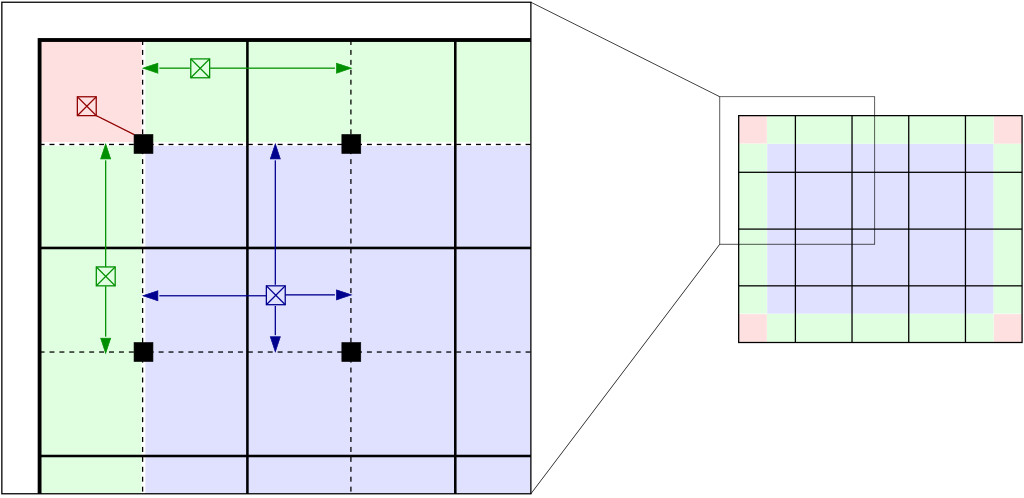
\includegraphics[width=10cm]{ahe-interploation.png}
                \caption{sample an interpolation}\label{1-a}
                \end{minipage}
        \end{figure}
        \subparagraph{}
        如图1-a所示,图像被分割为了$4\times 5$个区域(图中黑色实线分割区域),每个区域的中心,即为样本点。对于其他任意点,我们根据其位置,分为三种情况:\\
        \begin{description}
          \item[棱角(红色区域)] 使用原本区域的直方图均衡化映射
          \item[边缘(绿色区域)] 对x轴或y轴上临近瘔2个样本点使用线性插值计算映射
          \item[中心(蓝色区域)] 对周围4个样本点使用双线性插值计算映射
        \end{description}
        \subparagraph{}
        比如对中心区域的一个点P(x,y),它在原图中的灰度值为i,记距离它最近左上、右上、左下、右下的样本点的坐标分别为:\\
        \begin{center}
          $(x_{-},y_{-})$、$(x_{+},y_{-})$、$(x_{-},y_{+})$、$(x_{+},y_{+})$\\
        \end{center}
        对应的直方图映射函数分别为\\
        \begin{center}
        $m_{--}(x)$、$m_{-+}(x)$、$m_{+-}(x)$、$m_{++}(x)$\\
        \end{center}
        则P点的灰度值用双线性插值表示为:
        \begin{equation}
            Gray(P) = a[bm_{--}(i)+(1-b)m_{+-}(i)]+[1-a][bm_{-+}(i)+(1-b)m_{++}(i)]
        \end{equation}
        其中
        \begin{equation*}
            a = \frac{y-y_{-}}{y_{+}-y_{-}},  b = \frac{x-x_{-}}{x_{+}-x_{-}}
        \end{equation*}
        \subparagraph{}
        对于边缘和棱角的像素点,将更加简单。通过插值计算,大大加快了ahe的效率,又不会降低算法的质量。
    \section{结果}
        \paragraph{}我选用了经典的灰度图片:”天安门“测试了我写的算法,在我电脑上的运行时间不超过2秒,结果令人满意\\
        \paragraph{}
         \begin{figure}[htbp!]
                \begin{minipage}[t]{0.5\linewidth}\centering
                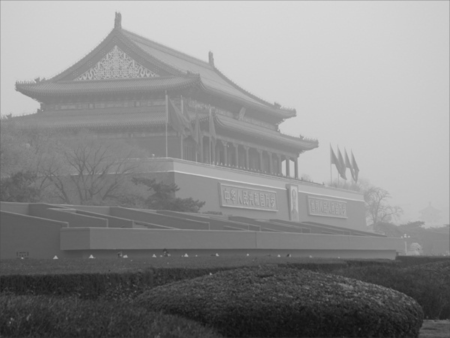
\includegraphics[width=6cm]{test.png}
                \caption{input image}\label{2-a}
                \end{minipage}
                \begin{minipage}[t]{0.5\linewidth}\centering
                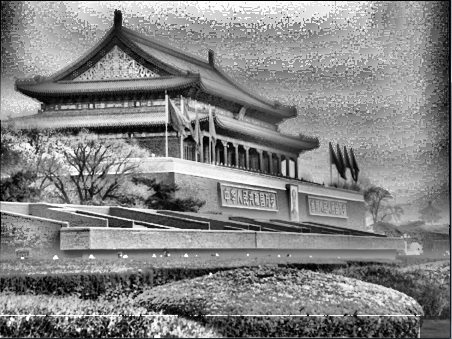
\includegraphics[width=6cm]{result.png}
                \caption{ahe result}\label{2-b}
                \end{minipage}
        \end{figure}
   
\end{document}
